% begin module max-min-ex2
\begin{frame}
\begin{example}[Example 2, p. 205]
Consider the function $y = x^2$.
\begin{columns}[c]
\column{.5\textwidth}
\ 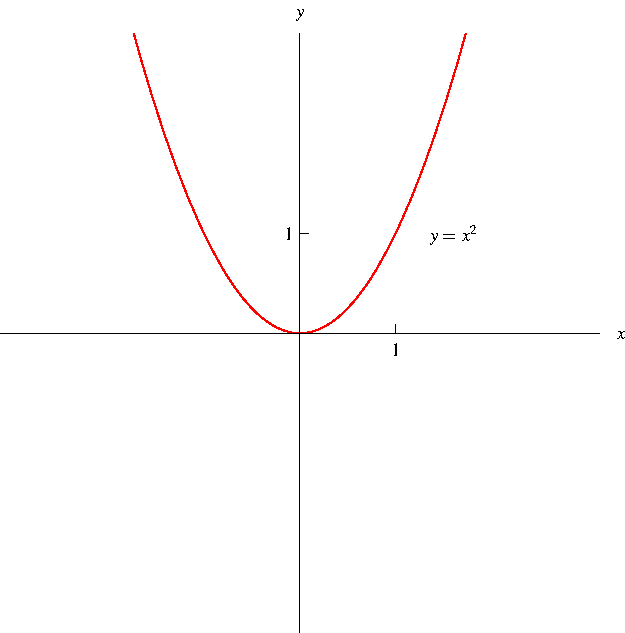
\includegraphics[width=6cm]{maxima-minima/pictures/01-02-xsquared.pdf}%
\column{.5\textwidth}
\begin{itemize}
\item<1-| alert@2-3>  Absolute maximum: \uncover<3->{None}
\item<1-| alert@4-5>  Absolute minimum: \uncover<5->{at 0}
\item<1-| alert@6-7>  Local maximum: \uncover<7->{None}
\item<1-| alert@8-9>  Local minimum: \uncover<9->{at 0}
\end{itemize}
\end{columns}
\end{example}
\end{frame}
% end module max-min-ex2
